\chapter*{Introduction}
\addcontentsline{toc}{chapter}{Introduction}

Consider a simple\footnote{An undirected graph with no self loops and at most 1 edge between any two nodes} graph $G$. How many colours do you need to colour each edge such that no edges which touch
have the same colour? What if no edges which touch some common edge can have the same colour?
Erd\H{o}s and Nešetřil conjectured that you only need $1.25\Delta(G)^2$ colours but
the best known proof only shows an upper bound of $1.772\Delta(G)^2$ colours. In this thesis
we show how we can bring this bound down to $1.73\Delta(G)^2$ by introducing a novel framework
which is a modification of Razborov's flag algebras. We also apply this new framework
to some other open problems including a bounded-degree version of the
Erd\H{o}s' pentagon conjecture.

\section*{Strong Edge Colouring}
\addcontentsline{toc}{section}{Strong Edge Colouring}
\label{sec:intro_strong_edge_coloring}

An edge colouring of a simple graph $G$ is an assignment $c\colon E(G) \to [k]$
for some $k\in\N$. Such a colouring is \textit{proper} if no two incident\footnote{Have a vertex in common}
edges have the same colour.
A colouring is \textit{strong} if no edges which share a common incident edge have
the same colour. Put differently, proper colouring requires edges at distance 1 to have distinct
colours and strong colouring extends this to distance 2.
In figure \ref{fig:proper-strong-example} we see an example of a non-proper colouring,
a proper (but not strong) colouring and a strong colouring of $C_5$.

\begin{figure}[h]
    \centering
    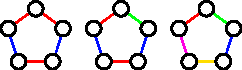
\includegraphics[scale=1.5]{proper-strong-example}
    \caption{Non-Proper, Proper \& Strong Edge Colourings}
    \label{fig:proper-strong-example}
\end{figure}

The \textit{chromatic index} of $G$, denoted $\chi'(G)$, is the minimum $k$ such that a proper edge
colouring of $G$ with $k$ colours exists. The \textit{strong chromatic index} $\chi'_s(G)$
is the corresponding minimum number of colours required for a strong edge colouring.

Vizing's theorem is a well known result which tells us $\chi'(G)$ almost exactly in terms of
the max degree of the graph $\Delta(G)$:
\begin{knowntheorem}[Vizing, 1965 \cite{Vizing_1965}]
    $\Delta(G) \leq \chi'(G) \leq \Delta(G) + 1$.
\end{knowntheorem}
Erd\H{o}s and Nešetřil conjectured in 1985 that
the strong chromatic index can also be bounded precisely by a function of the max degree:
\begin{knownconjecture}[Erd\H{o}s and Nešetřil \cite{faudreeInducedMatchingsBipartite1989}]
    \label{conj:intro_erdos_nesetril}
    $\chi'_s(G) \leq \frac{5}{4}\Delta(G)^2$.
\end{knownconjecture}
A greedy argument shows a bound of $\chi'(G) \leq 2\Delta(G)^2 + o(\Delta(G)^2)$ but it wasn't until
1997 that Molloy and Reed broke the $2\Delta(G)^2$ barrier \cite{molloyBoundStrongChromatic1997}.
A series of papers have since made progress on bringing this bound down closer to $\frac{5}{4}\Delta(G)^2$.

For $\Delta(G)$ large enough we have the following theorems:
\begin{enumerate}
  \item \textit{Molloy \& Reed, 1997} \cite{molloyBoundStrongChromatic1997}:
        $\chi'_s(G) \leq 1.998\Delta(G)^2$.
  \item \textit{Bruhn \& Joos, 2015} \cite{bruhnStrongerBoundStrong2018}:
        $\chi'_s(G) \leq 1.93\Delta(G)^2$.
  \item \textit{Bonamy, Perrett \& Postle, 2018} \cite{bonamyColouringGraphsSparse2018}:
        $\chi'_s(G) \leq 1.835\Delta(G)^2$.
  \item \textit{Hurley, de Verclos \& Kang, 2022} \cite{hurleyImprovedProcedureColouring2022}:
        $\chi'_s(G) \leq 1.772\Delta(G)^2$.
\end{enumerate}

In this thesis we will show how we brought this bound down even further to $1.73\Delta(G)^2$:
\begin{knowntheorem}
    For $\Delta(G)$ large enough we have
    $\chi'_s(G) \leq 1.73\Delta(G)^2$.
\end{knowntheorem}

The 1997 paper by Molloy \& Reed introduced a method for strong edge colouring we call the
\textit{2 step strategy}:
\begin{enumerate}
    \item Find an upper bound for the \textit{strong neighbourhood density} of $G$ in terms of
        $\Delta(G)$.
    \item Use a probabilistic colouring method which uses the previous bound to achieve a colouring
        with a low number of colours.
\end{enumerate}
This method has been modified by the papers which followed the Molloy \& Reed paper but this
strategy has remained the core idea. We will look at this strategy in more detail (including
defining strong neighbourhood density) in chapter \ref{chap:strong_edge_colouring}.
For this thesis we focus on the first step, using the second step as a black box. We will
find a new, lower, upper-bound on the strong neighbourhood density and hence achieve our
new colouring number.

\section*{Flag Algebras}
\addcontentsline{toc}{section}{Flag Algebras}

Step 1 of the 2-step strategy
asks us to find an upper bound on the strong neighbourhood density. The strong neighbourhood
density belongs to a broad family of density functions which ask: "How many copies of some
structure $F$ do we find in some larger structure $G$, expressed as a real number $\in [0,1]$"?
These density functions usually count the number of copies of $F$ in $G$, then normalise by the
maximum possible number of such copies.
For example, the density of edges in some graph $G$ is $|E(G)|/\binom{|G|}{2}$.

Bounding densities
is a common problem in combinatorics and in 2007 Razborov \cite{razborovFlagAlgebras2007}
introduced a framework called \textit{flag algebras}
which can be used to prove asymptotic results about densities in various combinatorial settings.
These flag algebras are defined very generally in terms of finite model theory in \cite{razborovFlagAlgebras2007} but we focus on their use with respect to simple graphs.

We give a brief flavour of flag algebras here but defer a full exposition until
chapter \ref{chap:classic_flags}.

\subsection*{A motivating example}
\label{sec:motivating_example}

As a reminder, for a graph $G$ and subset of vertices $U\subseteq V(G)$ the \textit{induced subgraph}
$G[U]$ is the subgraph of $G$ consisting of the vertices in $U$ and all edges between them.
We can then define the \textit{induced count} of $F$ in $G$, denoted $c(F; G)$, as
the number of subsets $U\subseteq V(G)$ such that $G[U] \cong F$. Then we define the
\textit{induced density} as $p(F; G) := c(F; G) / \binom{|G|}{|F|}$.

\begin{note}
    $p(F; G)$ is precisely the same as the probability that $G[U] \cong F$ if
    $U \subseteq V(G)$ is a uniformly random subset of size $|F|$.
\end{note}

What are some simple algebraic relationships between small subgraphs?
One thing that seems intuitive is that the density of edges in $G$ plus the density
of non-edges in $G$ is precisely 1. Similarly the densities of all possible graphs on
3 vertices is also 1.
\begin{align*}
    p(\edge; G) + p(\nonedge; G) &= 1\\
    p(\triangleflag; G)
    + p(\triangletwoedge; G)
    + p(\triangleoneedge; G)
    + p(\triangleempty; G) &= 1
\end{align*}

The density of edges is the probability that if we pick a pair of vertices that there is an
edge between them. We can relate this to the densities of graphs on 3 vertices by remarking
that sampling a pair of vertices uniformly at random can be done by first sampling a
triple of vertices at random, and then sampling 2 of those 3 uniformly again. This gives
us the following relation:
\[
    p(\edge; G) = 
    p(\triangleflag; G)
    + \frac{2}{3}p(\triangletwoedge; G)
    + \frac{1}{3}p(\triangleoneedge; G)
    + 0\cdot p(\triangleempty; G)
\]
A similar thought experiment relating sampling two pairs uniformly at random to sampling 4
vertices and then splitting the 4 randomly into two halves tells us:
\[
    p(\edge; G)^2 \sim p(\kfour; G) + \frac{2}{3}\left(p(\kfourmone; G) + p(\cfour; G)\right)
        + \frac{1}{3}\left(p(\kfourmtwo; G) + p(\kfourbucket; G) + p(\kfourtwopair; G)\right)
\]

Simplifying our notation then we might arrive at a symbolic algebra which has relations
like
\begin{align*}
    \edge + \nonedge &= 1\\
    \triangleflag
    + \triangletwoedge
    + \triangleoneedge
    + \triangleempty &= 1\\
    \edge &=
    \triangleflag
    + \frac{2}{3}\triangletwoedge
    + \frac{1}{3}\triangleoneedge\\
    \edge^2 &=
    \kfour + \frac{2}{3}(\kfourmone + \cfour)
        + \frac{1}{3}(\kfourmtwo + \kfourbucket + \kfourtwopair).
\end{align*}

We can then prove results with simple symbolic manipulation: In a triangle free graph
we would have $\triangleflag = 0$, hence
\[
    \edge = \frac{2}{3}\triangletwoedge + \frac{1}{3}\triangleoneedge \leq
    \frac{2}{3}(\triangletwoedge + \triangleoneedge)
    \leq \frac{2}{3}(\triangleflag + \triangletwoedge + \triangleoneedge + \triangleempty)
    \leq \frac{2}{3}
\]
as flags are non-negative. This (given all the formal definitions and proofs we've deferred)
is a formal proof
that $p(\edge; G) \leq \frac{2}{3}$ for any triangle free graph. The best possible result
says that $p(\edge; G) \leq \frac{1}{2}$ and is known as
\textit{Mantel's theorem} \cite{Mantel_1910}. This is
also easily proved with flag algebras which is seen in chapter \ref{chap:classic_flags}.

\subsection*{Computer Search}

One of the most (if not \textit{the most}) important aspects of flag algebras is that
they lend themselves very well to computer search methods.
The flag algebras allow us to prove results using only simple symbol manipulation in a very
tractable way; All details of the structures at play are abstracted out, only algebraic relations
between real numbers remains. We then have several tools at our disposal, in particular
linear combinations of flag inequalities can capture complex counting arguments, and
we will see later an operator on the algebra which enables us to use Cauchy-Schwarz style
arguments.

In practice we use the \textit{semidefinite method} to optimise some objective function
over the algebra, and due to duality this gives us a rigorous proof of an upper bound on our
function.
We will see in section \ref{sec:semidefinite_method} how we construct the semidefinite program,
and how we can interpret the dual solutions in a more human understandable way.

\section*{Local Flags}
\addcontentsline{toc}{section}{Local Flags}

One might be tempted to try to apply these flag algebras directly to our strong neighbourhood
density problem but in practice this problem doesn't fit well into the flag algebra model.
In particular, Razborov's flag algebras are constructed to work well with density functions
like the induced density function $p(F; G) = c(F; G)/\binom{|G|}{|F|}$ which have a
denominator which is $\Theta(|G|^{|F|})$. This is convenient if we are trying to prove
a bound on some function which is polynomial in $|G|$
(e.g. Mantel's theorem says the number of edges is $\leq \frac{1}{4}|G|^2$). But what if
we want to prove a bound on a function which is polynomial in some other function
of $G$? e.g. The \hyperref[conj:intro_erdos_nesetril]{Erd\H{o}s-Nešetřil Conjecture}
wants to bound $\chi'_s(G)$ with a polynomial in $\Delta(G).$ This does not lend itself
to the same methods.

Instead, we can define a new "density" function which instead normalises our induced
count by a different denominator, one which captures the graph parameter we want to measure
our count "relative to". The idea to build a new algebra from a modified density function was
originally explored by de Verclos in 2020\footnote{In unpublished notes}; He theorised what this
algebra could look like in a specific case and modified some classic flag algebra\footnote{An
implementation he wrote himself: \url{https://crates.io/crates/flag-algebra}} software to show that this method likely could improve on the
Erd\H{o}s and Nešetřil conjecture. This thesis evolves and formalises this idea and
then applies it concretely.

In particular, in chapter \ref{chap:local_flags} we introduce a
new \textit{local density function} and a concept we call a \textit{local flag}.
We show that, under certain conditions, these local flags also form a nice algebra
with which we can apply the semidefinite method to prove bounds. We then apply this new
method to several problems, including the 
\hyperref[conj:intro_erdos_nesetril]{Erd\H{o}s-Nešetřil Conjecture}.

\section*{Results}
\addcontentsline{toc}{section}{Results}

Using this new framework we have made progress on several open problems:
\begin{itemize}
    \item In chapter \ref{chap:pentagon_conjecture} we show a "warmup" application of the new framework by making progress on
        a bounded degree version of the famous Erd\H{o}s pentagon conjecture \cite{erdos_pentagon_1984}.
        We show how a straightforward application of the local flags method makes non-trivial
        progress towards proving the conjecture, and show that a slightly more complex application
        then gets even closer to the full result.
        This problem was chosen as the original conjecture was first proven using
        the classic flag algebras (\cite{hatamiNumberPentagonsTrianglefree2013},
        \cite{grzesikMaximumNumberFivecycles2012}).
    \item In chapter \ref{chap:strong_edge_colouring} then we apply this new framework to make progress on the
        \hyperref[conj:intro_erdos_nesetril]{Erd\H{o}s-Nešetřil Conjecture}, achieving the best-yet
        bound of $\chi'_s(G) \lesssim 1.73\Delta(G)^2$.
    \item At the end of chapter \ref{chap:strong_edge_colouring} we alter the method to make
        the first progress on the special bipartite version of this conjecture, showing that
        if $G$ is bipartite then we have the bound $\chi'_s(G) \lesssim 1.6254\Delta(G)^2$.
\end{itemize}
